\section{Deep Inelastic Scattering}\label{sec:DIS}
We have given a somewhat formal introduction of Quantum Chromodynamics as the theory of strong interactions. However, as this description only applies to the fundamental constituents, namely the quarks and gluons, we need to connect this formalism to scattering amplitudes involving particles that are composited of quarks and gluons. These composited particles are what particle physicists call \emph{hadrons}. Hadrons are categorized into two families: baryons, made of an odd number of quarks – usually three quarks – and mesons, made of an even number of quarks—usually one quark and one antiquark. Protons and neutrons are examples of baryons and pions are an example of a meson. For more detail on the classification of particles, see \cite{PhysRevD.98.030001}.

\medskip
As a non-abelian gauge theory, QCD has the peculiar behaviour of asymptotic freedom, and as described above, this is due to the anti-screening of gluons. As the coupling is \textquote{small} at high energies, the intuitive approach is to use perturbation theory. However, before that can be accomplished in a meaningful way, we have to define exactly what we are to expand.

Asymptotic freedom effectively separates the strong interaction into two regimes: A perturbative regime -- $\alpha_s$ is smaller than unity -- where we can expand using standard field theory methods, and a non-perturbative regime where we are unable to calculate. Unfortunately, we can not ignore the non-perturbative regime in real-life scattering processes. Thus, we need a method where we can unite both regimes into useful observables. To achieve this we need the concept of \emph{factorization}, which allows for separation of the low and high energy regime. This separation is made at an arbitrary energy scale, called the \emph{factorization scale}, and just like the renormalization scale observables can not depend on it. This naturally leads to evolution equations that describe the behaviour of the non-perturbative part as a function of the energy scale.

\medskip
The original, and still one of the most powerful, test of perturbative QCD is the Bjorken scaling in \emph{deep inelastic scattering} (DIS). Here a hadron is probed by a highly relativistic lepton, breaking up the hadron, creating additional hadrons in the final state. Only the lepton needs to be measured in the final state, meaning the final state hadrons can be integrated out. At sufficiently high energies the DIS experiments indicated the lepton scattered of point-like particles. This led Richard Feynman to postulate that hadrons were composite objects made up of fundamental constituents, which he called partons. This was the birth of what is called the \emph{parton model} \cite{Feynman:1970fm}. 

James Bjorken was the first to formalise the parton model in DIS \cite{PhysRev.179.1547}, where he was able to predict the behaviour of the hadronic system without any fundamental Lagrangian or knowledge of the hadron structure. He parametrized the process using so-called \emph{structure functions}. In the high energy limit, he showed that these structure functions only depended on a dimensionless scaling variable. 

In \cref{sec:DIS and Parton model} we will take a closer look at this parametrization and via a calculation verify Bjorken scaling in the parton model before we in \cref{sec:QCD and Collinear factorization} include QCD effects and move on to the more precise concept of factorization. 

%%%%%%%%%%%%%%%%%%%%%%%%%%%%%%%%%%%%%%%%%%%
\subsection{DIS and the Parton Model}\label{sec:DIS and Parton model}
Protons are in the parton model envisioned as extended objects, made up of partons and glued together by their mutual interactions. Of course, the partons are the quarks and gluons of quantum chromodynamics, but we will proceed without referring to this fact just yet. 

The essential assumption of the parton model is that at high energies and momentum transfer, the electron scatters of \textquote{free} point-like particles. This seems like a strange assumption, as the strong interaction between the constituents is what make protons bound objects in the first place. To justify this assumption, we can use basic principles from special relativity. We consider the inclusive process of electron--proton scattering at high energy, where the interaction goes through an exchange of a virtual photon with momentum $q$. In the centre-of-mass frame, two key concepts happen to the proton: since it is ultra-relativistic the proton is Lorentz contracted in the direction of travel, and the internal interactions are time-dilated. 

Therefore, if the time the electron uses to traverse the proton is shorter than the dilated time of interaction, the electron effectively scatters of non-interacting partons. This is known as the impulse approximation. Also, when the momentum transfer is very high, the virtual photon becomes short-lived. Then, if the parton density is sufficiently low, the electron can only interact with one single parton. Since the partons do not interact between themselves during this period, each carries a definite fraction $\xi$ of the proton's momentum $P$. With this picture, it is possible to calculate the electron--parton interaction using perturbation theory without considering the proton as a whole.


The high energy inelastic process is therefore separated into a short-distance scattering part---the interaction between the photon and one of the partons---called the \emph{hard} part, and a long-distance---everything inside the proton---\emph{soft} part. Because of the different time scales of these two effects, one assumes that there is no quantum mechanical interference between them. The hadronic cross-section may thus be calculated by combining probabilities, rather than amplitudes. We define parton distribution functions $f_{i/h}(\xi)$ to describe the probability that a parton of type $i$ has a fraction $\xi$ of the hadrons momentum. 

\begin{figure}
    \centering
    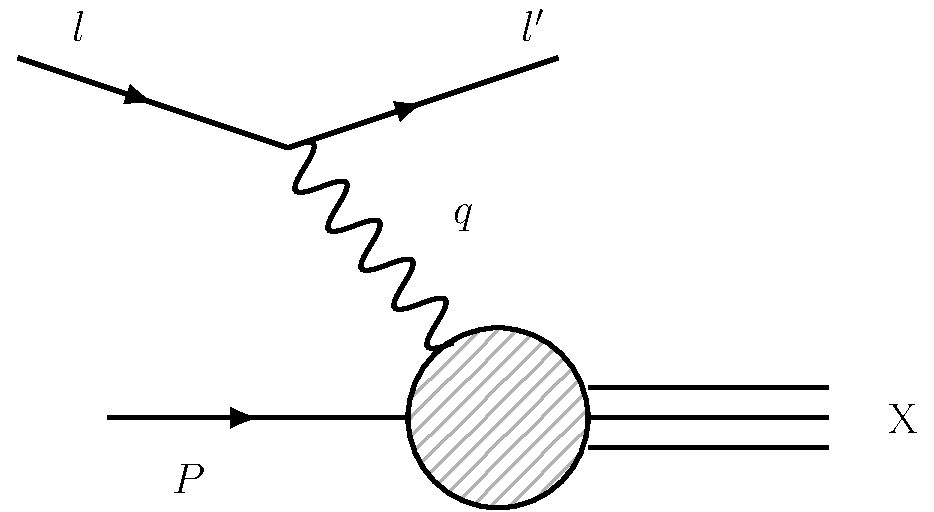
\includegraphics[scale=0.4]{Figures/DIS.pdf}
    \caption{Kinematics of deep inelastic electron--proton scattering}
    \label{fig:Deep Inelastic Scattering}
\end{figure}
\medskip

\subsection*{Kinematics}
We consider the scattering of a high energy electron off a proton target, via the exchange of a virtual photon (see \cref{fig:Deep Inelastic Scattering}). The full treatment would involve weak interactions, but for our purposes we only consider the electromagnetic interaction. We lable the incoming and outgoing electron momenta with $l^{\mu}$ and $l'^{\mu}$ respectively, the momentum of the proton by $P^{\mu}$ and the momentum transfer by the photon $q^{\mu}=l^{\mu}-l'^{\mu}$. We will assume that the mass of the electron and the proton constituents are negligible compared to the scale of the process. The centre-of-mass energy squared is then
\begin{align}
    s=(P+l)^{2}=m_{p}^{2}+2P\cdot l\,,
\end{align}
where $m_{p}$ is the mass of the proton. It follows that the momentum transfer squared is given by
\begin{align}
    q^{2}=2E_{l}E_{l'}(\cos\theta_{ll'}-1)\leq 0\,.
\end{align}
Therefore, it is useful to instead define $Q^{2}\equiv-q^{2}\geq 0$. The invariant mass of the final state $X$ is given by
\begin{align}
    m_{X}^{2}=(P+q)^{2}=m_{p}^{2}+2P\cdot q-Q^{2}\,.
\end{align}
In order to have \emph{deep} and \emph{inelastic} scattering, we must have the requirement that $Q^{2}\gg m_{p}^{2}$---\,the momentum transfer is so large that the proton target is very much excited\,---\,and inelastically $m_{X}^{2}\gg m_{p}^{2}$. 

The two independent Lorentz invariants for the hadron system are $Q^{2}$ and $P\cdot q$, but it is convenient to define additional invariant variables
\begin{align}
    x_{B}&=\frac{Q^{2}}{2P\cdot q}\,,\label{eq:Bjorken-x}
    \\
    y&=\frac{P\cdot q}{P\cdot l}=\frac{Q^{2}}{x_{B}(s-m_{p}^{2})}\,.
\end{align}
Here $x_{B}$ is called \emph{Bjorken-x}, which we from now will only denote by $x$. Kinematically $x$ is restricted to the range $Q^{2}/s+Q^{2}\leq x \leq 1$, neglecting terms of $\mathcal{O}(m_{p}^{2}/Q^{2})$. In the parton model we will find that $x$ gives an estimate for the hadron's momentum fraction that is carried by the struck parton. In the rest frame of the proton $y$ is the fractional energy loss of the electron, but it is not an independent variable since it is given by $Q^{2}$ and $x$.



\subsection*{Factorization and Bjorken Scaling}
From the above picture, the parton model describes DIS without the strong interaction participating, as all strong effects have been absorbed into the proton. Consequently, the proton is like a black box, where we have no idea of its structure, except that we can extract a parton from it.

Before we write down the amplitude and differential cross-section for this process, we must define some relations for current matrix elements. A fermion current is $j^{\mu}(z)=\bar{\psi}(z)\gamma^{\mu}\psi(z)$, with $\psi(z)$ the fermion field. A generic current matrix element for a fermion is then given by
\begin{align}\label{eq:generic current matrix element}
    \bra{k'}j^{\mu}(z)\ket{k}=\Bar{u}(k')\gamma^{\mu}u(k)\,e^{i(k'-k)\cdot z}\,,
\end{align}
where we used $z$ as space-time variable in order to avoid confusion with the Bjorken-$x$. The relation in \cref{eq:generic current matrix element} can be derived using the expansion of the fermion fields in terms of creation and annihilation operators. Thus, a shorthand for the spinor product $\Bar{u}(k')\gamma^{\mu}u(k)$ coming out of matrix elements is just the current matrix element at space-time point $z=0$, i.e. 
\begin{align}
    \bra{k'}j^{\mu}(0)\ket{k}=\Bar{u}(k')\gamma^{\mu}u(k)\,.
\end{align}
Then we can write the amplitude for DIS as
\begin{align}
    \mathcal{M}=\bra{l'}\,j_{L}^{\mu}\,\ket{l}\bra{X}\,j_{H}^{\nu}\,\ket{P}\,D_{\mu\nu}(q)\,,
\end{align}
where $D_{\mu\nu}(q)$ is just the regular photon propagator, see \cref{eq:photon propagator without gauge choice}. The differential cross section then takes the form
\begin{align}
    d\sigma&=\frac{1}{4\,P\cdot l}\frac{d^{3}l'}{(2\pi)^{3}\,2E_{l'}}\sum_{X}\int\frac{d^{3}p_{X}}{(2\pi)^{3}\,2E_{X}}(2\pi)^{4}\delta^{(4)}(P+l-p_{X}-l)|\mathcal{M}|^{2}\nonumber\,,
\end{align}
giving
\begin{align}\label{eq:DIS differential cross section}
    E_{l'}\frac{d\sigma}{d^{3}l'}&=\frac{2}{s-m_{p}^{2}}\frac{\alpha^{2}}{Q^{4}}L_{\mu\nu}W^{\mu\nu}\,,
\end{align}
where $\alpha$ is the fine structure constant. As we only consider photon exchange, the lepton tensor is completely determined by QED
\begin{align}
    L_{\mu\nu}=\frac{1}{2}\text{tr}[\slashed{l'}\gamma_{\mu}\slashed{l}\gamma_{\nu}]=2\big(l_{\mu}l'_{\nu}+l_{\nu}l'_{\mu}-g_{\mu\nu}l\cdot l'\big)\,.
\end{align}
In contrast, the hadronic tensor contains all the information about the interaction between the electromagnetic current $j_{H}^{\mu}$ and the proton $P$
\begin{align}
    W^{\mu\nu}&=4\pi^{3}\sum_{X}\int\frac{d^{3}p_{X}}{(2\pi)^{3}\,2E_{X}}\delta^{(4)}(P+q-p_{X})\,\bra{P}\,j^{\dag\,\mu}(0)\,\ket{X}\bra{X}\,j^{\nu}(0)\,\ket{P}\nonumber
    \\
    &=\frac{1}{4\pi}\int d^{4}z\,\sum_{X}\int\frac{d^{3}p_{X}}{(2\pi)^{3}\,2E_{X}}\,e^{iz\cdot(P+q-p_{X})}\,\bra{P}\,j^{\dagger\,\mu}(0)\,\ket{X}\bra{X}\,j^{\nu}(0)\,\ket{P}\,,\nonumber
\end{align}
where we used the integral representation of the four dimensional delta function. Further, we can use the translation operator
\begin{align}\label{eq:translation operator}
    \,\bra{P}\,j^{\dagger\,\mu}(0)\,\ket{X}e^{iz\cdot(P-p_{X})}&=\,\bra{P}e^{iz\cdot\hat{P}}\,j^{\dagger\,\mu}(0)\,e^{-iz\cdot\hat{P}}\ket{X}\nonumber
    \\
    &=\bra{P}\,j^{\dagger\,\mu}(z)\,\ket{X}\,,
\end{align}
and integrate out a complete set of states by the use of the completeness relation:
\begin{align}\label{eq:complete set of states}
    \sum_{X}\int\frac{d^{3}p_{X}}{(2\pi)^{3}\,2E_{X}}\ket{X}\bra{X}=\boldsymbol{1}\,.
\end{align}
The hadronic tensor can then be written as
\begin{align}\label{eq:hadronic tensor in terms of currents}
    W^{\mu\nu}=\frac{1}{4\pi}\int d^{4}z\,e^{iq\cdot z}\bra{P}\,j^{\dagger\,\mu}(z)j^{\nu}(0)\ket{P}\,.
\end{align}

This tensor can now be decomposed in terms of tensors that governs the kinematics times scalar functions. To do this, we use that the electromagnetic current is conserved, $\partial_{\mu}j^{\mu}=0$, so that the hadronic tensor satisfies the Ward identity $q_{\mu}W^{\mu\nu}=0$. Further, using that the strong interaction is parity invariant and $W^{\mu\nu}$ is hermitian, the most general form of the hadronic tensor for unpolarized protons can be written as
\begin{align}\label{eq:1stparametrized hadronic tensor}
    W^{\mu\nu}=\Big(-g^{\mu\nu}+\frac{q^{\mu}q^{\nu}}{q^{2}}\Big)F_{1}(x,Q^{2})+\Big(P^{\mu}+\frac{1}{2x}q^{\mu}\Big)\Big(P^{\nu}+\frac{1}{2x}q^{\nu}\Big)\frac{1}{P\cdot q}F_{2}(x,Q^{2})\,.
\end{align}
The scalar functions $F_{1}$ and $F_{2}$ are the structure functions we alluded to earlier. They contain the information of the hadron structure as \textquote{seen} by the virtual photon. Combining this with the leptonic tensor we find that
\begin{align}
    L_{\mu\nu}W^{\mu\nu}=\frac{2Q^{2}}{xy^{2}}\Big[\Big(1-y+\frac{y^{2}}{2}\Big)2xF_{1}(x,Q^{2})+(1-y)\big(F_{2}(x,Q^{2})-2xF_{1}(x,Q^{2})\big)\Big]\,.
\end{align}
Plugging this into \cref{eq:DIS differential cross section}, and neglecting terms of $\mathcal{O}( m_{p}^{2}/Q^{2})$ gives the unpolarized electron--proton DIS cross section
\begin{align}\label{eq:full differential DIS}
    \frac{d^{2}\sigma}{dxdy}=\frac{4\pi\alpha^{2}s}{Q^{4}}\Big[\Big(1-y+\frac{y^{2}}{2}\Big)2xF_{1}(x,Q^{2})+(1-y)\big(F_{2}(x,Q^{2})-2xF_{1}(x,Q^{2})\big)\Big]\,.
\end{align}
To find a parton model prediction for the behaviour of the structure functions, we calculate the partonic equivalent of $\cref{eq:full differential DIS}$. Thus, we are only interested in electron--quark scattering, $e^{-}(l)q(p)\rightarrow e^{-}(l')q(p')$. By using the Mandelstam variables
\begin{align}
    \hat{s}=(l+p)^{2}\,,\hspace{0.5cm}\hat{t}=(l-l')\,,\hspace{0.5cm}\hat{u}=(p-l')\,,
\end{align}
it is straightforward to show that the spin/colour averaged amplitude takes the form
\begin{align}
    \langle\, |\mathcal{M}|^{2}\rangle = 2Q_{q}^{2}e^{4}\,\frac{\hat{s}^{2}+\hat{u}^{2}}{\hat{t}^{2}}\,,
\end{align}
where $Q_{q}$ is the fractional charge of the quark. Using the standard result for the differential cross section for massless $2\rightarrow 2$ scattering:
\begin{align}
    \frac{d\hat{\sigma}}{d\hat{t}}=\frac{1}{16\pi\hat{s}^{2}} \langle\, |\mathcal{M}|^{2}\rangle\,,
\end{align}
which after some rewriting will give the partonic differential cross section
\begin{align}
    \frac{d\hat{\sigma}}{dy}=Q_{q}^{2}\frac{4\pi\alpha^{2}\hat{s}}{Q^{4}}\Big(1-y+\frac{y^{2}}{2}\Big)\,.
\end{align}
In order to relate the hard cross section with the full cross section, we define the quark momentum as a fraction of the proton momentum,
\begin{align}
    p^{\mu}=\xi P^{\mu}\,, \hspace{0.8cm}0<\xi<1\,,
\end{align}
such that $\hat{s}=\xi s$. If we approximate with an on-shell constraint for the outgoing quark, we find that 
\begin{align}
    p'^{2}=(p+q)^{2}=2\xi P\cdot q -Q^{2}=0\,,
\end{align}
implying that $\xi=x$. The on-shell constraint fixes the momentum fraction to equal the Bjorken variable, but this is of course not a general result. The Bjorken-$x$ is a kinematical constraint defining the process, while $\xi$ is just a momentum fraction that is independent of the process. To obtain a double differential cross-section as in \cref{eq:full differential DIS}, we simply use that 
\begin{align}
    \int_{0}^{1}dx\,\delta(x-\xi)=1\,,
\end{align}
and write
\begin{align}\label{eq:partonic differential DIS}
    \frac{d^{3}\hat{\sigma}}{dxdyd\xi}=Q_{q}^{2}\frac{4\pi\alpha^{2}s}{Q^{4}}\Big(1-y+\frac{y^{2}}{2}\Big)\,\xi\,\delta(x-\xi)\,.
\end{align}
We can now use the parton model interpretation of $f_{q}(\xi)$ as a probability and convolute it with the partonic part. To find the electron--proton differential cross section we simply integrate over all possible fraction $\xi$ and sum over quark flavour
\begin{align}\label{eq:parton model factorization}
    \frac{d^{2}\sigma}{dxdy}&=\sum_{q}\int_{0}^{1}d\xi\,f_{q}(\xi)\,\frac{d^{3}\hat{\sigma}}{dxdyd\xi}\nonumber
    \\
    &=\frac{4\pi\alpha^{2}s}{Q^{4}}\Big(1-y+\frac{y^{2}}{2}\Big)\,\sum_{q}Q_{q}^{2}\,x\,f_{q}(x)\,.
\end{align}
Then if we compare \cref{eq:parton model factorization} with \cref{eq:full differential DIS} we see that the proton structure functions in this simple model is given by
\begin{align}\label{eq:proton structure functions F_2 and F_1}
    F_{2}(x)=2xF_{1}(x)&=\sum_{q}Q_{q}^{2}\,x\,f_{q}(x)\,.
\end{align}
This result shows that in the regime where $Q^{2}$ is very large, we have that the structure functions only depend on the Bjorken-$x$. This is what is called \emph{Bjorken scaling}, and the result $F_{2}=2xF_{1}$ is known as the \emph{Callan-Gross relation}. The Callan-Gross relation follows from the spin-$1/2$ nature of quarks and was later confirmed by structure function measurements. These predictions made the parton model an intriguing model to further explore the structure of hadrons.

In \cref{eq:parton model factorization} we convoluted the partonic cross section with the parton distributions resulting in a hadronic cross section. Therefore, we can also define quark structure functions that we can convolute with the parton distribution, giving the proton structure functions. We see that if we define
\begin{align}
    \hat{F}_{2}=Q_{q}^{2}\,x\,\delta(1-x)\,,\label{eq:quark structure function hat_F2}
    \\
    \hat{F}_{1}=\frac{1}{2}Q_{q}^{2}\,\delta(1-x)\,,\label{eq:quark structure function hat_F1}
\end{align}
we can write the parton model factorization formulas for the proton structure functions as,
\begin{align}
    F_{2}(x)&=\sum_{q}\int_{x}^{1}d\xi\,f_{q}(\xi)\hat{F}_{2}\Big(\frac{x}{\xi}\Big)=\sum_{q}Q_{q}^{2}\,x\,f_{q}(x)\label{eq:collinear factorization parton model F_2}\,,
    \\
    F_{1}(x)&=\sum_{q}\int_{x}^{1}\frac{d\xi}{\xi}f_{q}(\xi)\hat{F}_{1}\Big(\frac{x}{\xi}\Big)=\frac{1}{2}\sum_{q}Q_{q}^{2}f_{q}(x)\label{eq:collinear factorization parton model F_1}\,,
\end{align}
giving the same result as above. The integration bound follows from $x/\xi\leq 1$. In the same manner the differential cross section can be written in the following way:
\begin{align}
     d\sigma(x,Q^{2})&=\sum_{q}\int_{x}^{1}d\xi\,f_{q}(\xi)\,d\hat{\sigma}\Big(\frac{x}{\xi},Q^{2}\Big)\,,
    \\
\end{align}
which is known as \emph{collinear factorization} of DIS in the parton model. An important point to make is that the above factorized integrals are convolutions defined in \emph{Mellin Space}, see \cref{sec:Appendix Mellin Transform}. Mellin transformations and their properties are very useful in studying QCD, which we will lay out in more detail in \cref{chap:Resummation in QCD}.

The collinear terminology used here refers to the fact that we have only considered the case where the quark momentum is in the same direction as the proton. We should, therefore, point out that $f_{q}(\xi)$ is formally defined as
\begin{align}
    f_{q}(\xi)=\int d^{2}k_{\perp}f_{q}(\xi,k_{\perp})\,,
\end{align}
where the transverse momentum dependence has been integrated out. It should also be pointed out that this is only valid as we only measure the final state lepton. If we wanted to take into account the final state hadrons we would have to use \emph{transverse momentum distributions} (TMDs), which is much more complicated. In this chapter we will only consider processes, like DIS and Drell-Yan, where the final state hadrons are integrated out.

\medskip
We have seen that the parton model result can give predictions that have been confirmed by experiments, but it is a phenomenological model and is not a formal treatment of the strong interaction. However, the concept of factorization is exactly what makes one take a field theoretical approach to hadronic scattering processes. Including QCD into the parton model results in interactions between the partons, and the assumption of free partons does not hold anymore. Therefore, the above factorization formulas are invalid and we must make a more precise definition of factorization in QCD. To this end, we will consider the case of QCD corrections to the DIS process in the next section. 

\medskip
To end this section we will make a brief remark about the difference between structure functions and parton distribution functions. The structure functions appeared when we parametrized the hadronic tensor, which is process dependent. That is, if we considered DIS neutrino scattering, the structure functions would change as we, in that case, considered $W$ or $Z$ boson exchange. The main idea behind factorization is that, inside the structure functions, we can factorize out the proton content from the process dependent part. The factorization ansatz in \cref{eq:parton model factorization} is required to be valid for any process, meaning that the PDFs are universal. Thus, the PDFs can be extracted from DIS electron--proton scattering experiments and re-used in another experiment like DIS neutrino--proton scattering and proton--proton collisions at the LHC.

%%%%%%%%%%%%%%%%%%%%%%%%%%%%%%%%%%%%%%%%%
\subsection{Collinear Factorization in QCD}\label{sec:QCD and Collinear factorization}
In \cref{sec:DIS and Parton model} we saw that the observables in the parton model could be written on a factorized form. The crucial element of that result is the assumption that the quark momentum is a fraction of the proton's momentum, $p^{\mu}=\xi P^{\mu}$. This is in general not true, as the quark will also have transverse components. To highlight the validity of the parton model assumption it is useful to use \emph{light-cone coordinates}, see \cref{sec:Appendix Light-cone coordinates}. 

By considering the case where the proton has no transverse momentum components, the general form of the proton and parton momenta can be parametrized as
\begin{align}
    P^{\mu}=\Big(P^{+},\frac{m_{p}^{2}}{2P^{+}},0_{\perp}\Big)\,,\hspace{1cm}
    p^{\mu}=(p^{+},p^{-},p_{\perp})\,.
\end{align}
It is safe to assume that in the protons rest frame, the distribution of partons is isotropic, and that the components of the parton momentum is of the order of the proton mass. We are free to choose frame, so by choosing the frame where $P^{+}\rightarrow \infty$, the only remaining component of the proton momentum is its plus-component. It is also hard to imagine that the partons will not follow the proton along this direction---at least if we assume no gluon radiation---so we find that
\begin{align}
    P^{\mu}=(P^{+},0^{-},0_{\perp})\,,\hspace{1cm}
    p^{\mu}\approx(p^{+},0^{-},0_{\perp})\,.
\end{align}
This is what is called the \emph{infinite momentum frame} (IMF), and the partons transverse components has been neglected compared to the plus-component, $p^{+}\gg p_{\perp}\sim m_{p}$. We can now assume that the struck quark has a fraction $\xi$ of the proton's momentum, giving that in the infinite momentum frame the parton momentum is fully collinear to the proton momentum
\begin{align}
    p^{\mu}=\xi P^{\mu}\,,
\end{align}
which is the result we used for the parton model in \cref{sec:DIS and Parton model}. 

However, if the struck parton is a quark that has just emitted a gluon this is no longer necessarily true, and we will need a more general parametrization of the momenta. We can use $p^{+}=\xi P^{+}$ to parametrize the parton momentum in terms of the large plus-component $P^{+}$
\begin{align}\label{eq:light-cone parametrization}
    P^{\mu}=\Big(P^{+},\frac{m_{p}^{2}}{2P^{+}},0_{\perp}\Big)\,,\hspace{1cm}p^{\mu}=\Big(\xi P^{+},\frac{p^{2}+p_{\perp}^{2}}{2\xi P^{+}},p_{\perp}\Big)\,,
\end{align}
which reproduces the infinite momentum frame limit for $p^{2},p_{\perp}^{2},m_{p}^{2}\ll P^{+}$. In turn the photon momentum can be parametrized as
\begin{align}\label{eq:light-cone photon momenta}
    q^{\mu}=\Big(0,\frac{Q^{2}}{2xP^{+}},q_{\perp}\Big)\,,
\end{align}
where $-q^{2}=q_{\perp}^{2}=Q^{2}$ and $P\cdot q=Q^{2}/2x$, meaning that this choice reproduces the known kinematics in DIS, given in \cref{eq:Bjorken-x}. Not only does light-cone coordinates formalise the parton model assumption of fully collinear partons in the IMF, but as we will later see it is in this formalism that the parton model has it's closest relation to field theory. In the following calculations we will parametrize all momenta as in \cref{eq:light-cone parametrization}.

\medskip
In the parton model calculation we found that the structure functions scale, i.e. $F(x,Q^{2})\rightarrow F(x)$ in the Bjorken limit $Q^{2}\rightarrow \infty$. By including QCD into this picture, $F(x,Q^{2})$ will have terms that are proportional to $\ln{Q^{2}}$, i.e. we have logarithmic breaking of Bjorken scaling. The key point is that the original quark can emit a gluon before being struck by the photon and will acquire a transverse component that can not be neglected. As we shall see below, when integrating over the intermediate quark momentum, the integral over this transverse component extends up to the kinematic limit  $Q^{2}$, leading to this logarithmic dependancy of $Q^{2}$. 

Factorization in QCD is therefore the determination of at which point the emitted gluon belongs to the soft part or the hard part of the scattering. The correct way to determine this\,---\,at least in the collinear case\,---is to define a separation in terms of an energy scale $\mu_{F}$ (factorization scale). Thus, if the gluon is emitted at a scale lower than $\mu_{F}$ it is part of the PDF (soft part) and if it is emitted at a scale larger than $\mu_F$ it is part of the partonic process (hard part). The all order proof of factorization in QCD is beyond the scope of this thesis, so here we will investigate the $\mathcal{O}(\alpha_s)$ correction to DIS and see how that changes the parton model factorization.

\medskip
\subsection*{One gluon emission}
\begin{figure}
    \centering
    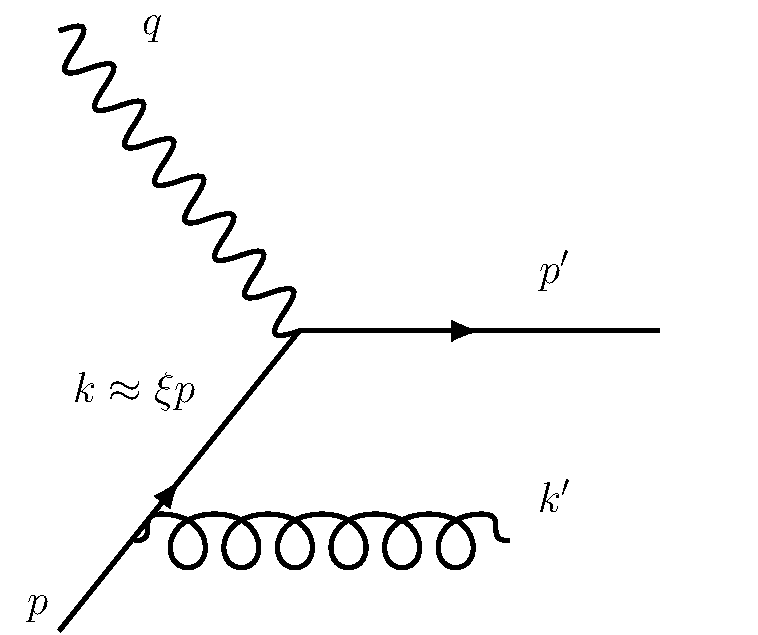
\includegraphics[scale=0.4]{Figures/gluonemissionDIS.pdf}
    \caption{Gluon emission from initial quark.}
    \label{fig:DISgluonemission}
\end{figure}

At NLO there are two real gluon diagrams and three virtual gluon diagrams in DIS. The real diagrams are emission from initial and final quark line, while the virtual diagrams are self energy diagrams of the initial and final state together with exchange of a gluon between the initial and final quark lines.
However, we will only consider gluon emission from the initial quark line, given in \cref{fig:DISgluonemission}. The reason for this is that we will choose to work with gluons in light-cone gauge, and in this gauge this is the only diagram that gives a logarithmic divergence. The other diagrams will give finite results that are unimportant for the current discussion and will be omitted for brevity.

\medskip
The way to proceed is to investigate corrections to the hadronic tensor and extract the structure functions from it. The proton strucure functions were in the parton model written as a convolution between the PDF and the quark structure functions, see \cref{eq:collinear factorization parton model F_2} and \cref{eq:collinear factorization parton model F_1}. The hadronic tensor can also be written on this convoluted form
\begin{align}
    W^{\mu\nu}(x,Q^{2})=\sum_{q}\int_{x}^{1}\frac{d\xi}{\xi}f_{q}(\xi)\hat{W}^{\mu\nu}\Big(\frac{x}{\xi},Q^{2}\Big)\,,
\end{align}
where $\hat{W}^{\mu\nu}$ refers to the partonic part that are calculable in perturbation theory. Thus, we will calculate $\hat{W}^{\mu\nu}$ up to $\mathcal{O}(\alpha_s)$ and extract $\hat{F}_{2}$ from it, enabling us to compare with \cref{eq:collinear factorization parton model F_2} to see the effect it has on the PDF.

In \cref{eq:1stparametrized hadronic tensor} we parametrized the hadronic tensor as
\begin{align}
    W^{\mu\nu}=\Big(-g^{\mu\nu}+\frac{q^{\mu}q^{\nu}}{q^{2}}\Big)F_{1}(x,Q^{2})+\Big(P^{\mu}+\frac{1}{2x}q^{\mu}\Big)\Big(P^{\nu}+\frac{1}{2x}q^{\nu}\Big)\frac{1}{P\cdot q}F_{2}(x,Q^{2})\,.
\end{align}
However, in higher order calculations there is an alternative parametrization that comes in handy when we want to extract the structure functions. Hence, we define normalized basis vectors (factors and terms $\mathcal{O}(m_{p}^{2}/Q^{2})$ are as usual neglected)
\begin{align}\label{eq:basis vectors}
    \hat{q}^{\mu}&\equiv\frac{q^{\mu}}{Q}\, ,\hspace{1cm}\hat{t}^{\mu}\equiv\frac{1}{Q}(q^{\mu}+2xP^{\mu})\,.
\end{align}
These basis vector satisfy: $\hat{q}\cdot\hat{t}=0$, $\hat{q}^{2}=-1$ and $\hat{t}^{2}=1$, meaning that $\hat{q}$ is spacelike and $\hat{t}$ is timelike. With respect to these basis vectors one can also define a transverse tensor
\begin{align}
    g_{\perp}^{\mu\nu}\equiv g^{\mu\nu}+\hat{q}^{\mu}\hat{q}^{\nu}-\hat{t}^{\mu}\hat{t}^{\nu}\,,
\end{align}
from which the following relations follow
\begin{align}
    \hat{t}_{\mu}g_{\perp}^{\mu\nu}&=0
    \\
    \hat{q}_{\mu}g_{\perp}^{\mu\nu}&=0
    \\
    g_{\perp}^{\mu\nu}g_{\perp\,\mu\nu}&=2\,,
\end{align}
making it consistent with \cref{eq:trasnversal tensor}. With these definitions it is straightforward to rewrite the hadronic tensor as
\begin{align}\label{eq:2ndparametrized hadronic tensor}
    W^{\mu\nu}(x,Q^{2})=-g_{\perp}^{\mu\nu}F_{1}(x,Q^{2})+\frac{\hat{t}^{\mu}\hat{t}^{\nu}}{2x}\big(F_{2}(x,Q^{2})-2xF_{1}(x,Q^{2})\big)\,,
\end{align}
from which the structure functions can be extracted by applying appropriate tensors on the hadronic tensor
\begin{align}
    F_{1}&=-\frac{1}{2}g_{\perp}^{\mu\nu}W_{\mu\nu}\,,\label{eq:extracting F_1}
    \\
    F_{2}&=x(2\hat{t}^{\mu}\hat{t}^{\nu}-g_{\perp}^{\mu\nu})W_{\mu\nu}\,.\label{eq:extracting F_2}
\end{align}
For the $F_{2}$ projection is is useful to note that $(2\hat{t}^{\mu}\hat{t}^{\nu}-g_{\perp}^{\mu\nu})g_{\mu\nu}=0$, which will cancel all terms involving $g^{\mu\nu}$ in the Dirac traces. 

The amplitude for the gluon emission in \cref{fig:DISgluonemission}, is given by
\begin{align}
    \mathcal{M}^{\mu}=-igQ_{q}t^{a}\varepsilon_{\beta}^{*}(k')\,\bar{u}(p')\,\gamma^{\mu}\frac{\slashed{k}}{k^{2}}\gamma^{\beta}\,u(p)\,.
\end{align}
We average over incoming spin and colour, sum over final spin, colour and gluon polarization,
\begin{align}
    \langle\,|\mathcal{M}|^{2}\rangle^{\mu\nu}&=\frac{1}{N_{s}N_{c}}\sum_{a,b}\sum_{\text{spin}}\sum_{\text{pol}}\big(|\mathcal{M}|^{2}\big)^{\mu\nu}\,\nonumber
    \\
    &=\frac{C_{F}}{N_s}Q_{q}^{2}g^{2}\frac{1}{k^{4}}\sum_{\text{pol}}\varepsilon_{\alpha}(k')\varepsilon_{\beta}^{*}(k')\,\text{tr}[\gamma^{\nu}\slashed{p}'\gamma^{\mu}\slashed{k}\gamma^{\alpha}\slashed{p}\gamma^{\beta}\slashed{k}]\,.
\end{align}
We can then use the gluon polarization sum in the light-cone gauge (see \cref{eq:gluon polarization sum light-cone gauge})
\begin{align}
    \sum_{\text{pol}}\varepsilon_{\alpha}(k')\varepsilon_{\beta}^{*}(k')&=-g_{\alpha\beta}+\frac{k'_{\alpha}\,n_{-\,\beta}}{k'^{+}}+\frac{k'_{\beta}\,n_{-\,\alpha}}{k'^{+}}\,,
\end{align}
which will give the following expression for the Dirac trace
\begin{align}
    \sum_{\text{pol}}\varepsilon_{\alpha}(k')\varepsilon_{\beta}^{*}(k')\,\text{tr}[\gamma^{\nu}\slashed{p}'\gamma^{\mu}\slashed{k}\gamma^{\alpha}\slashed{p}\gamma^{\beta}\slashed{k}]=&-\text{tr}[\gamma^{\nu}\slashed{p}'\gamma^{\mu}\slashed{k}\gamma^{\alpha}\slashed{p}\gamma_{\alpha}\slashed{k}]+\frac{1}{k'^{+}}\text{tr}[\gamma^{\nu}\slashed{p}'\gamma^{\mu}\slashed{k}\slashed{k}'\slashed{p}\gamma^{+}\slashed{k}]\nonumber
    \\
    &+\frac{1}{k'^{+}}\text{tr}[\gamma^{\nu}\slashed{p}'\gamma^{\mu}\slashed{k}\gamma^{+}\slashed{p}\slashed{k}'\slashed{k}]\,.\nonumber
\end{align}

These traces can be calculated using the relations given in \cref{sec:Appendix Dirac gamma matrices}, but it is tedious so we will just write out the main steps. The first trace can be simplified to
\begin{align}
    \text{tr}[\gamma^{\nu}\slashed{p}'\gamma^{\mu}\slashed{k}\gamma^{\alpha}\slashed{p}\gamma_{\alpha}\slashed{k}]=-4p\cdot k\,\text{tr}[\gamma^{\nu}\slashed{p}'\gamma^{\mu}\slashed{k}]+2k^{2}\,\text{tr}[\gamma^{\nu}\slashed{p}'\gamma^{\mu}\slashed{p}]\,,
\end{align}
and the last two traces can first be simplified by using that $k'=p-k$, giving
\begin{align}
    \text{tr}[\gamma^{\nu}\slashed{p}'\gamma^{\mu}\slashed{k}\slashed{k}'\slashed{p}\gamma^{+}\slashed{k}]&=-k^{2}\,\text{tr}[\gamma^{\nu}\slashed{p}'\gamma^{\mu}\slashed{p}\gamma^{+}\slashed{k}]\,,
    \\
    \text{tr}[\gamma^{\nu}\slashed{p}'\gamma^{\mu}\slashed{k}\gamma^{+}\slashed{p}\slashed{k}'\slashed{k}]&=-k^{2}\,\text{tr}[\gamma^{\nu}\slashed{p}'\gamma^{\mu}\slashed{k}\gamma^{+}\slashed{p}]\,,
\end{align}
where the sum of these two traces can be rewritten as
\begin{align}
    -k^{2}\text{tr}[\gamma^{\nu}\slashed{p}'\gamma^{\mu}(\slashed{k}+\slashed{p})\gamma^{+}(\slashed{p}+\slashed{k})]=&-2(k^{+}+p^{+})k^{2}\,\text{tr}[\gamma^{\nu}\slashed{p}'\gamma^{\mu}\slashed{k}]\nonumber
    \\
    &-2(k^{+}+p^{+})k^{2}\,\text{tr}[\gamma^{\nu}\slashed{p}'\gamma^{\mu}\slashed{p}]\nonumber
    \\
    &+k^{2}(k^{2}+2p\cdot k)\text{tr}[\gamma^{\nu}\slashed{p}'\gamma^{\mu}\gamma^{+}]\,.\nonumber
\end{align}
Collecting all terms and using the cyclic property of the trace, we find that the sum of all traces can be written as
\begin{align}
    \sum\text{tr}(...)=&\,\Big(4p\cdot k-2k^{2}\frac{k^{+}+p^{+}}{k^{+}-p^{+}}\Big)\text{tr}[\slashed{k}\gamma^{\mu}\slashed{p}'\gamma^{\nu}]\nonumber
    \\
    &-2k^{2}\Big(1+\frac{k^{+}+p^{+}}{k^{+}-p^{+}}\Big)\text{tr}[\slashed{p}\gamma^{\mu}\slashed{p}'\gamma^{\nu}]\nonumber
    \\
    &+\frac{k^{2}}{k^{+}-p^{+}}\big(k^{2}+2p\cdot k\big)\text{tr}[\slashed{n}_{-}\gamma^{\mu}\slashed{p}'\gamma^{\nu}]\,,\nonumber
\end{align}
where we used that $\gamma^{+}=\slashed{n}_{-}$, such that all the traces take the same form. For generic vectors, $a^{\mu}$ and $b^{\mu}$, these traces evaluate to\footnote{See \cref{sec:Appendix Dirac gamma matrices} for more detail on traces.}
\begin{align}\label{eq:tracetrace}
    \text{tr}[\slashed{a}\gamma^{\mu}\slashed{b}\gamma^{\nu}]=4(a^{\mu}b^{\nu}+a^{\nu}b^{\mu}-g^{\mu\nu}a\cdot b)\,.
\end{align}
Hence, we write the averaged amplitude as
\begin{align}\label{eq:ththehte amp}
    \langle\,|\mathcal{M}|^{2}\rangle^{\mu\nu}=\frac{C_{F}}{N_s}Q_{q}^{2}g^{2}\frac{1}{k^{4}}\sum\text{tr}(...)\,.
\end{align}


To calculate $\hat{W}^{\mu\nu}$, we must integrate over the final state particles, giving
\begin{align}
    \hat{W}^{\mu\nu}=\frac{1}{4\pi}\int d\mathcal{P}_{2}\,\langle\, |\mathcal{M}|^{2}\rangle \,,
\end{align}
where $4\pi$ comes from the normalization in \cref{eq:hadronic tensor in terms of currents}. The n-body phase space for on-shell massless particles is given by \cref{eq:n-body phase space}, so the two-body phase space takes the form
\begin{align}\label{eq:DIS differential phase space}
    d\mathcal{P}_{2}&=\int\frac{d^{4}k'}{(2\pi)^{3}}\frac{d^{4}p'}{(2\pi)^{3}}\,\delta^{+}(k'^{2})\delta^{+}(p'^{2})(2\pi)^{4}\delta^{(4)}(p+q-k'-p')\nonumber
    \\
    &=\frac{1}{4\pi^{2}}\int d^{4}k\,\delta^{+}\big((p-k)^{2}\big)\delta^{+}\big((k+q)^{2}\big)\,,
\end{align}
where we use that $\delta^{+}(k'^{2})\equiv \delta(k'^{2})\theta(k'^{+})$\footnote{In light-cone coordinates the usual Heaviside function $\theta(k^{0})$ is replaced by $\theta(k^{+})$.}.
Note that we work explicitly in four dimensions, which mean we will not use dimensional regularization in this calculation. For the Drell-Yan process (see \cref{sec:Drell-Yan Hadronic Cross Section}), we will perform a full calculation using dimensional regularization, but for physical intuition it is more useful to use momentum cutoff in DIS.  

\medskip
In the partonic system we assume that the original quark has no transverse components and move in the plus direction, the virtual\footnote{All quarks are kind of virtual, but this is common terminology in scattering processes to specify that it is intermediate, i.e. propagating and off-shell.} quark on the other hand may have large transverse components due to the radiation of a gluon from the original quark. Thus, the relevant momenta in the partonic system is given by:
\begin{align}
    p^{\mu}&=(p^{+},0^{-},0_{\perp})\,,
    \\
    k^{\mu}&=\Big(\xi p^{+},\frac{k_{\perp}^{2}-|k^{2}|}{2\xi p^{+}},k_{\perp}\Big)\,,
    \\
    q^{\mu}&=\Big(0,\frac{Q^{2}}{2xp^{+}},q_{\perp}\Big)\,,
\end{align}
where we used that $k^{2}=-|k^{2}|$ because the intermediate quark is virtual. The arguments of the delta functions in \cref{eq:DIS differential phase space} is given by
\begin{align}
    (p-k)^{2}&=-2p\cdot k-|k^{2}|=-\frac{1}{\xi}\big(k_{\perp}^{2}-(1-\xi)|k^{2}|\big)\,,
    \\
    (k+q)^{2}&=2k\cdot q-|k^{2}|-Q^{2}=2P\cdot q\Big(\xi-x-\frac{|k^{2}|+2k_{\perp}\cdot q_{\perp}}{2P\cdot q}\Big)\,,
\end{align}
and the differential is given by
\begin{align}
    d^{4}k=dk^{+}dk^{-}d^{2}k_{\perp}=\frac{1}{4\xi}d\xi dk^{2}dk_{\perp}^{2}d\theta\,,
\end{align}
with $0<\theta<\pi$. Inserting these expression into \cref{eq:DIS differential phase space}, we get
\begin{align}
     d\mathcal{P}_{2}&=\frac{1}{(4\pi)^{2}P\cdot q}\int d\xi dk^{2}dk_{\perp}^{2}d\theta \hspace{2mm}\delta\big(k_{\perp}^{2}-(1-\xi)|k^{2}|\big)\,\delta\Big(\xi-x-\frac{|k^{2}|+2k_{\perp}\cdot q_{\perp}}{2P\cdot q}\Big)\,.
\end{align}

Now, there is no a priori reason why the transverse momentum (or equivalently $|k^{2}|$) should be small, but in the second delta function the effect of these are damped by $P\cdot q\sim Q^{2}$ so we proceed by neglecting this term. This again fixes $\xi=x$ in the final integration. We are actually jumping ahead here, but with a more thorough analysis it can be shown that this is in fact the case \cite{Ellis1996QCDAC}. The first delta function fixes $k_{\perp}^{2}=(1-\xi)|k^{2}|$, so we can just use it directly to rewrite the averaged amplitude in \cref{eq:ththehte amp}, giving
\begin{align}
    \langle\, |\mathcal{M}|^{2}\rangle^{\mu\nu}=&4\pi C_{F}\,Q_{q}^{2}\,\alpha_{s}\frac{1}{|k^{2}|}\Big[\frac{1}{\xi}\frac{1+\xi^{2}}{1-\xi}\big(8k^{(\mu}p'^{\nu)}-4g^{\mu\nu}k\cdot p'\big)\nonumber
    \\
    &+\frac{1}{1-\xi}\big(8p^{(\mu}p'^{\nu)}-4g^{\mu\nu}p\cdot p'\big) + \frac{1}{1-\xi}\frac{|k^{2}|}{p^{+}}\big(8n_{-}^{(\mu}p'^{\nu)}-4g^{\mu\nu}p'^{+}\big)\Big]\,.
\end{align}
where we have evaluated the traces using \cref{eq:tracetrace} and for notational simplicity defined $a^{(\mu}b^{\nu)}=(a^{\mu}b^{\nu}+a^{\nu}b^{\mu})/2$.

Let us then finally use \cref{eq:extracting F_2} to project out $\hat{F}_{2}$,
\begin{align}
    \hat{F}_{2}=\int d\mathcal{P}_{2}\,\,x(\hat{t}^{\mu}\hat{t}^{\nu}-g_{\perp}^{\mu\nu})\,\langle\, |\mathcal{M}|^{2}\rangle_{\mu\nu}\,.
\end{align}
In the following we will only list the divergent term as the finite ones are unimportant for this discussion. For the contraction with the matrix element we use that $p'=k+q$ and the basis vector $\hat{t}$ is found from \cref{eq:basis vectors}. Putting everything together is messy, but after the effect of the delta functions the divergent part takes the form\footnote{For a more detailed derivation of this term, see \cite{Ellis1996QCDAC}.}
\begin{align}\label{eq:divergent F_2}
    \hat{F}_{2}\,\big|_{\text{div}}=Q_{q}^{2}\frac{\alpha_s}{2\pi}\,xP_{q/q}(x)\int_{Q_{0}^{2}}^{Q^{2}}\frac{d|k^{2}|}{|k^{2}|}\,,
\end{align}
where the integral is regulated over $|k^{2}|$ in terms of a IR cut-off $Q_{0}^{2}$ and a UV cut-off $Q^{2}$, that follows from the kinematics. We have also defined a function $P_{q/q}(x)$, which is known as the \emph{quark--quark splitting function}
\begin{align}\label{eq:splitting function 1}
    P_{q/q}(x)=C_{F}\frac{1+x^{2}}{1-x}\,.
\end{align}
Its form is specific to the quark-quark-gluon vertex of QCD, and it represents the probability for a quark to split into another quark with momentum fraction $x$ and a gluon with momentum fraction $1-x$. Integrating \cref{eq:divergent F_2}, we find
\begin{align}\label{eq:divergent integrated F_2}
    \hat{F}_{2}\,\big|_{\text{div}}=Q_{q}^{2}\frac{\alpha_s}{2\pi}\,xP_{q/q}(x)\,\ln{\frac{Q^{2}}{Q_{0}^{2}}}\,.
\end{align}

If we include the leading order contribution given in \cref{eq:collinear factorization parton model F_2} and all finite terms, denoted $C_{q}(x)$, we have the quark structure function at $\mathcal{O}(\alpha_s)$
\begin{align}\label{eq:quark structure function correction}
    \hat{F}_{2}=Q_{q}^{2}\,x\Big(\delta(1-x)+\frac{\alpha_s}{2\pi}\big(P_{q/q}(x)\ln{\frac{Q^{2}}{Q_{0}^{2}}}+C_{q}(x)\big)\Big)\,.
\end{align}

The natural question that arises is how to interpret the divergence of the structure function. We observe that the singularity arises when the gluon is emitted fully collinear to the quark, i.e. $k_{\perp}=0$, and is therefore referred to as a \emph{collinear singularity}. To understand what is happening we need to realize that physically $k_{\perp}^{2}\rightarrow 0$ corresponds to a long-range part of the strong interaction which is not calculable in perturbation theory. Hence, if we use the PDFs to describe physics at long-range, we can convolute the structure function $\hat{F}_{2}$ with \textquote{bare} distributions $f_{q}^{0}$ to absorb the collinear singularity. This is a similar, but still different approach to the UV-renormalization procedure we discussed in \cref{sec:Renormalization}.

To get a clear understanding of how this is done we investigate the cut-off we made in \cref{eq:divergent F_2}. By imposing the IR cut-off we effectively integrate $k_{\perp}^{2}$ from $Q_{0}^{2}$ up to $Q^{2}$. Now, the kinematics of the process justifies the upper limit of $Q^{2}$ as $k_{\perp}$ is always smaller than or equal to $Q$\footnote{This follows from the fact that the transverse momentum of the gluon can not be larger than the scale of the process.}. However, in the IR-region there is no kinematical restriction on $k_{\perp}$. The lower cut-off ensures that the gluons with transverse momentum $k_{\perp}\leq Q_{0}$ is neglected from the hard part of the scattering. We can not drop these gluons entirely, so we absorb this part of the process into the PDF. We can then renormalize the PDF up to the arbitrary energy scale $\mu_F$.

\medskip
To obtain the proton structure function we convolute the quark structure function $\hat{F}_{2}$ of \cref{eq:quark structure function correction} with the bare PDF $f_{q}^{0}$ as we did for the parton model in \cref{eq:collinear factorization parton model F_2}, 
\begin{align}
    F_{2}(x,Q^{2})=\sum_{q}Q_{q}^{2}\,x\Big(f_{q}^{0}(x)+\frac{\alpha_s}{2\pi}\int_{x}^{1}\frac{d\xi}{\xi}f_{q}^{0}(\xi)\big[P_{q/q}\big(\frac{x}{\xi}\big)\ln{\frac{Q^{2}}{Q_{0}^{2}}}+C_{q}\big(\frac{x}{\xi}\big)\big]\Big)\,.
\end{align}
Then we can absorb the collinear singularities into the bare distribution at the factorization scale $\mu_F$, or in other words, we define a renormalized distribution
\begin{align}
    f_{q}(x,\mu_{F}^{2})=f_{q}^{0}(x)+\frac{\alpha_s}{2\pi}\int_{x}^{1}\frac{d\xi}{\xi}f_{q}^{0}(\xi)\big[P_{q/q}\big(\frac{x}{\xi}\big)\ln{\frac{\mu_{F}^{2}}{Q_{0}^{2}}}+C_{q}'\big(\frac{x}{\xi}\big)\big]\,,
\end{align}
which inserted into the expression for $F_{2}$ gives the finite result
\begin{align}\label{eq:renormalized F_2}
    F_{2}(x,Q^{2})=\sum_{q}Q_{q}^{2}\,x\int_{x}^{1}\frac{d\xi}{\xi}f_{q}(\xi,\mu_{F}^{2})\big[\delta\big(1-\frac{x}{\xi}\big)+\frac{\alpha_s}{2\pi}\Big(P_{q/q}\big(\frac{x}{\xi}\big)\ln{\frac{Q^{2}}{\mu_{F}^{2}}}+D_{q}\big(\frac{x}{\xi}\big)\Big)\big]\,.
\end{align}

This result says that we can choose an arbitrary energy scale $\mu_F$ to separate the process into two parts: a hard part where $k_{\perp}$ is larger than this scale, and a soft part where $k_{\perp}$ is smaller than this scale. Thus, we \textquote{hide} the divergence inside a part that were non-perturbative in the first place. We have alluded to this separation repeatedly and made this statement in the discussion of the parton model, but now we have extended that result to the correct framework of QCD. We also note that the only difference in QCD factorization and the parton model factorization is that the PDF and the hard part acquires a dependancy on the factorization scale. Although we have only demonstrated factorization to $\mathcal{O}(\alpha_S)$ in DIS, it has been proven to all orders in perturbation theory \cite{Collins:1989gx}. Another important feature of extending to QCD is that Bjorken-scaling is violated as $F_{2}$ is explicitly dependent on $Q^{2}$.

One important aspect of the renormalization procedure we have made here is that even though the factorization specifies a prescription of dealing with the logarithmic singularities, there is still an arbitrariness in the choice of the finite terms. In \cref{eq:renormalized F_2} we have that $D(x)=C(x)-C'(x)$, where $C'(x)$ is absorbed by the PDF and $D(x)$ is the terms that remains. However, we could have made another choice and absorbed all finite terms into the PDF, and the exact choice made is referred to as a \emph{factorization scheme}. The most common scheme is the $\overline{\text{MS}}$ scheme we mentioned in \cref{sec:Renormalization}, where the absorbed term is $C'=\ln 4\pi-\gamma_{E}$.

Due to the non-perturbative nature of long distance physics in QCD, the distributions $f_{q}(x,\mu_{F}^{2})$ are not directly   calculable from first principles, and must therefore be extracted from experiments or, more recently in lattice QCD. However, what can be calculated perturbatively is the dependence on the scale $\mu_{F}^{2}$. The proton structure function $F_{2}$ is an observable, meaning that it cannot depend on the choice of scale. This leads to the following requirement
\begin{align}
    \pdv{F_2}{\ln\mu_{F}^{2}}=0\,,
\end{align}
which leads to the following differential equation for the PDFs
\begin{align}\label{eq:1st evolution equation f_q}
    \pdv{}{\ln\mu_{F}^{2}}f_{q}(x,\mu_{F}^{2})=\frac{\alpha_{s}(\mu_{F}^{2})}{2\pi}\int_{x}^{1}\frac{d\xi}{\xi}P_{q/q}\big(\frac{x}{\xi}\big)\,f_{q}(\xi,\mu_{F}^{2})\,.
\end{align}
This evolution equation is similar to the $\beta$ function equation describing the evolution of the coupling $\alpha_{s}(\mu^{2})$, and is known as the Dokshitzer-Gribov-Altarelli-Parisi (DGLAP) equation. As it stands, this equation is only valid up to $\mathcal{O}(\alpha_s)$. To get an all order evolution equation we can expand the splitting function in the coupling,
\begin{align}
    P_{q/q}(x,\alpha_{s})=\sum_{n=0}^{\infty}\Big(\frac{\alpha_s}{2\pi}\Big)^{n+1}P_{q/q}^{(n)}(x)\,,
\end{align}
and write the evolution equation as
\begin{align}\label{eq:DGLAP equation}
    \pdv{}{\ln\mu_{F}^{2}}f_{q}(x,\mu_{F}^{2})=\int_{x}^{1}\frac{d\xi}{\xi}P_{q/q}\big(\frac{x}{\xi},\alpha_{s}(\mu_{F}^{2})\big)\,f_{q}(\xi,\mu_{F}^{2})\,,
\end{align}
where the higher order information is contained inside the splitting function. We can then identify the splitting function in \cref{eq:splitting function 1} and \cref{eq:1st evolution equation f_q} as the leading order splitting function $P_{q/q}^{(0)}$. For a more rigorous derivation of this generalization see \cite{Altarelli:1977zs}. 

In order to obtain a complete discussion of deep inelastic scattering in terms of parton distribution functions, there is one more ingredient that we have not considered. That is, we also need to consider the initial scattering of gluons. The $\mathcal{O}(\alpha_s)$ contribution for initial gluon scattering is through a t-channel boson-gluon fusion process. Following a similar line of argument as for the quark initial state this will lead to the gluon structure function
\begin{align}
    \hat{F}_{2}^{g}(x,Q^{2})=\sum_{q}Q_{q}^{2}\,x\,\frac{\alpha_s}{2\pi}\Big(P_{q/g}(x)\ln{\frac{Q^{2}}{Q_{0}^{2}}}+C_{g}(x)\Big)\,,
\end{align}
which is very similar to the quark structure function \cref{eq:quark structure function correction}, apart from the fact that at zeroth order in $\alpha_s$ there is no gluon radiation. The splitting function for this process is specific for the gluon-quark-quark vertex, and is given by
\begin{align}
    P_{q/g}(x)=\frac{1}{2}(x^{2}+(1-x)^{2})\,,
\end{align}
and is interpreted as the probability for a gluon to split into a quark with momentum fraction $x$ and another quark with momentum fraction $1-x$. 

As with the quark structure function we have to convolute the gluon structure function with a bare gluon distribution $f_{g}^{0}$, define a renormalized gluon distribution and add it to \cref{eq:renormalized F_2}. This is equivalent to redefining our renormalized quark parton distribution to also absorb the singular gluon term. Thus, we define
\begin{align}
    f_{q}(x,\mu_{F}^{2})=&f_{q}^{0}(x)+\frac{\alpha_s}{2\pi}\int_{x}^{1}\frac{d\xi}{\xi}f_{q}^{0}(\xi)\big[P_{q/q}\big(\frac{x}{\xi}\big)\ln{\frac{\mu_{F}^{2}}{Q_{0}^{2}}}+C'_{q}\big(\frac{x}{\xi}\big)\big]\nonumber
    \\
    &+\frac{\alpha_s}{2\pi}\int_{x}^{1}\frac{d\xi}{\xi}f_{g}^{0}(\xi)\big[P_{q/g}\big(\frac{x}{\xi}\big)\ln{\frac{\mu_{F}^{2}}{Q_{0}^{2}}}+C'_{g}\big(\frac{x}{\xi}\big)\big]\,.
\end{align}

Instead of writing the whole final expression out, let us be even more general and define hard functions with perturbative expansions
\begin{align}
    H_{q}(z)&=\sum_{n=0}^{\infty}\Big(\frac{\alpha_s}{2\pi}\Big)^{n}H_{q}^{(n)}(z)\,,
    \\
    H_{g}(z)&=\sum_{n=1}^{\infty}\Big(\frac{\alpha_s}{2\pi}\Big)^{n}H_{g}^{(n)}(z)\,.
\end{align}
where the $\mathcal{O}(\alpha_s)$ expansion is given by
\begin{align}
    H_{q}(z)&=H_{q}^{(0)}(z)+\frac{\alpha_s}{2\pi}H_{q}^{(1)}(z)=\delta(1-z)+\frac{\alpha_s}{2\pi}\Big(P_{q/q}^{(0)}(z)\ln{\frac{Q^{2}}{\mu_{F}^{2}}}+D_{q}(z)\Big)\,,
    \\
    H_{g}(z)&=\frac{\alpha_s}{2\pi}H_{g}^{(1)}(z)=\frac{\alpha_s}{2\pi}\Big(P_{q/g}^{(0)}(z)\ln{\frac{Q^{2}}{\mu_{F}^{2}}}+D_{g}(z)\Big)\,,
\end{align}
The collinear factorization formula for $F_2$ then takes the form
\begin{align}
    F_{2}(x,Q^{2})=&\sum_{q}Q_{q}^{2}\,x\int_{x}^{1}\frac{d\xi}{\xi}f_{q}(\xi,\mu_{F}^{2})H_{q}\big(\frac{x}{\xi},\frac{Q^{2}}{\mu_{F}^{2}},\alpha_{s}(\mu_{F}^{2})\big)\nonumber
    \\
    &+\sum_{q}Q_{q}^{2}\,x\int_{x}^{1}\frac{d\xi}{\xi}f_{g}(\xi,\mu_{F}^{2})H_{g}\big(\frac{x}{\xi},\frac{Q^{2}}{\mu_{F}^{2}},\alpha_{s}(\mu_{F}^{2})\big)\,.
\end{align}
To actually have a full description of collinear factorization in QCD we would need to find the factorization of $F_{1}$ as well. To find $F_{1}$ we would have to project it out as in \cref{eq:extracting F_1}, but we will not consider the specific calculation as it follows in the same manner as for $F_{2}$. 

\medskip
If one considered even higher order corrections we would encounter the additional splitting functions $P_{g/q}(x)$ and $P_{g/g}(x)$. $P_{g/q}(x)$ decribes the splitting of a quark into a gluon with momentum fraction $x$ and a quark with momentum fraction $1-x$, and similarly $P_{g/g}(z)$ describes the splitting of a gluon into a gluon with momentum fraction $x$ and another gluon with momentum fraction $1-x$. For completeness we list all splitting functions at leading order
\begin{align}
    P_{q/q}^{(0)}(x)&=C_{F}\frac{1+x^{2}}{1-x}\,,
    \\
    P_{q/g}^{(0)}(x)&=\frac{1}{2}(x^{2}+(1-x)^{2})\,,
    \\
    P_{g/q}^{(0)}(x)&=C_{F}\frac{1+(1-x)^{2}}{x}\,,
    \\
    P_{g/g}^{(0)}(x)&=2C_{A}\Big(\frac{x}{1-x}+\frac{1-x}{x}+x(1-x)\Big)\,.
\end{align}

We observe that $P_{q/q}(x)$ and $P_{g/g}(x)$ both have singular behaviour for $x\rightarrow 1$, so we will need to regularize these as well. This is done by using so-called \emph{plus distributions}, see \cref{sec:Appendix Plus Distributions}. We will encounter plus distributions in \cref{sec:Drell-Yan Hadronic Cross Section} as well, so it is useful to write down the regulated splitting functions. The regularized splitting functions are at leading order given by \cite{Altarelli:1977zs},
\begin{align}
    P_{q/q}^{(0)}(x)&=C_{F}\Big(\Big[\frac{1+x^{2}}{1-x}\Big]_{+}+\frac{3}{2}\delta(1-x)\Big)\,,\label{eq:qq splitting function}
    \\
    P_{g/g}^{(0)}(x)&=2C_{A}\Big(\Big[\frac{1+x^{2}}{1-x}\Big]_{+}+\frac{1-x}{x}+x(1-x)\Big)+\delta(1-x)\frac{(11C_{A}-2n_{f})}{6}\,,\label{eq:gg splitting function}
\end{align}
where $n_{f}$ is the number of quarks. 

This leads us to the end of our discussion of factorization in DIS. In \cref{sec:Drell-Yan Hadronic Cross Section} we will investigate one other process where factorization has been proven, namely the Drell-Yan process. But before we move on to the Drell-Yan cross section, there are some important details about parton distribution functions we have to discuss. That is, we can actually write PDFs as operator valued matrix elements, and use Wilson lines to render these gauge invariant. Not only that, but we can use the expansion of Wilson lines to describe gluon radiation from incoming partons. That is not to say that the universal distribtuins $f_{i/h}$ can be calculated in perturbation theory, but we can define parton-in-parton distributions that are calculable in perturbation theory. This is the topic of the next few chapters.

%%%%%%%%%%%%%%%%%%%%%%%%%%%%%%%%%%%%%%%%%
\subsection{Operator Definition for PDFs}\label{sec:Operator definition for Parton Distributions}
 

The interpretation of a parton distribution function as the probability of
finding a parton inside a proton with momentum fraction $\xi$ was
crucial in finding factorized formulas for QCD scattering observables. In quantum field
theory, we have that probabilities are matrix elements squared, so we would like to define the parton distribution functions as operator-valued matrix elements. In terms of operator definitions one can use them to prove the factorization properties of QCD, and one can also use them to include soft and collinear singularities. This last part is essential for what is called \emph{re-factorization} in QCD resummation, which we will come back to in \cref{chap:Resummation in QCD}. 

\medskip
In \cref{sec:DIS and Parton model} we found an expression for the hadronic tensor in terms of the electromagnetic currents in \cref{eq:hadronic tensor in terms of currents}. Here we will construct it diagrammatically such that we can extract the so-called \emph{quark correlator}, which are the building block for the parton distribution functions. The diagrammatic construction is illustrated in \cref{fig:Hadronic tensor}. The upper diagram pulls out a quark from the proton, which subsequently fragments into the final state $X$. Mathematically this is given by the matrix element
\begin{align}
    \mathcal{A}_{i}=\bra{X}\psi_{i}(0)\ket{P}\,.
\end{align}
Assuming a gauge interaction in $\mu$, the bottom diagram will give a quark in the final state. Then we will get the matrix element
\begin{align}
    \mathcal{A}^{\nu}=Q_{q}\bar{u}_{j}^{s}(k)\big(\gamma^{\nu}\big)^{ji}\bra{X}\psi_{i}(0)\ket{P}\,.
\end{align}
The squared matrix element for this part of the process can then be written as:
\begin{align}
    \big(|\mathcal{A}|^{2}\big)^{\mu\nu}=\sum_{q}Q_{q}^{2}\big[\gamma^{\mu}(\slashed{k}+m)\gamma^{\nu}\big]^{ji}\bra{P}\overline{\psi}_{j}(0)\ket{X}\bra{X}\psi_{i}(0)\ket{P}\,,
\end{align}
where we have used the spin sum rule
\begin{align}
    \sum_{s}u^{s}(k)\bar{u}^{s}(k)=\slashed{k}+m\,.
\end{align}
\begin{figure}
    \centering
    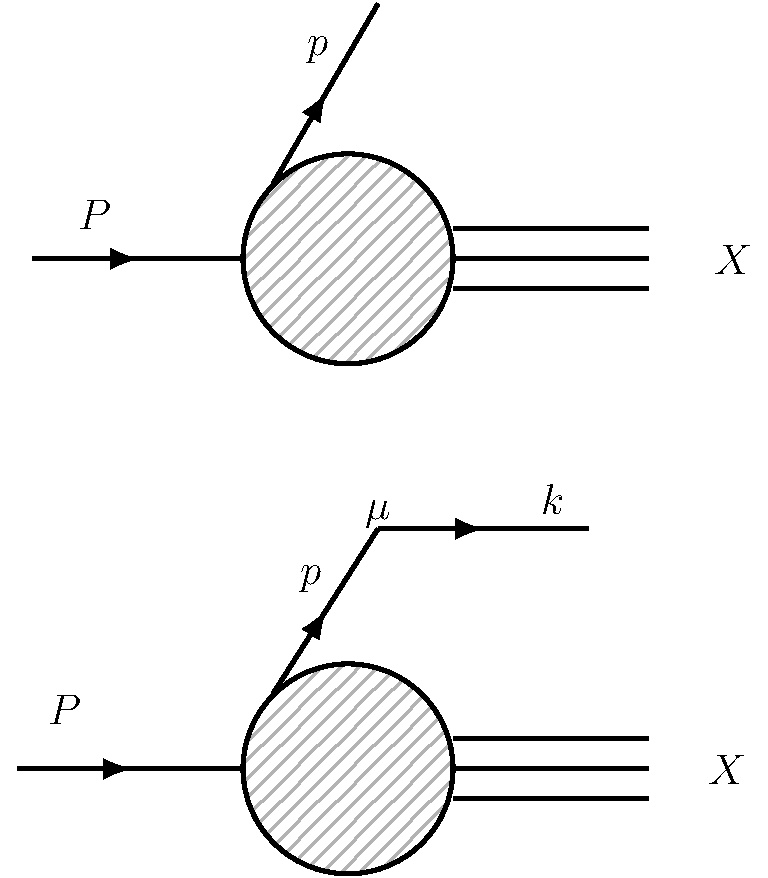
\includegraphics[scale=0.4]{Figures/HadronicTensor.pdf}
    \caption{Diagramatic construction of hadronic tensor}
    \label{fig:Hadronic tensor}
\end{figure}

To write down the hadronic tensor we integrate over the final states $X$ and $k$ and impose momentum conservation through a delta function. As usual, we use the exponential representation of the delta function, and the integral over $k$ will be made by using the on-shell condition, see \cref{eq:n-body phase space}
\begin{align}
    \int\frac{d^{3}k}{(2\pi)^{3}}\frac{1}{2k^{0}}=\int\frac{d^{4}k}{(2\pi)^{4}}2\pi\delta(k^{2}-m^{2})\theta(k^{0})\,,
\end{align}

Taking the quark to be massless, we find the hadronic tensor to take the form
\begin{align}
    W^{\mu\nu}&=4\pi^{3}\sum_{q}Q_{q}^{2}\sum_{X}\int\frac{d^{3}p_{X}}{(2\pi)^{3}2E_{X}}\int\frac{d^{3}k}{(2\pi)^{3}2k^{0}}\delta^{(4)}(P+q-k-p_{X})\nonumber
    \\
    &\hspace{0.8cm}\times\big(\gamma^{\mu}\slashed{k}\gamma^{\nu}\big)^{ji}\bra{P}\overline{\psi}_{j}(0)\ket{X}\bra{X}\psi_{i}(0)\ket{P}\nonumber
    \\
    &=4\pi^{3}\sum_{q}Q_{q}^{2}\sum_{X}\int\frac{d^{3}p_{X}}{(2\pi)^{3}2E_{X}}\int\frac{d^{4}k}{(2\pi)^{4}}2\pi\delta(k^{2})\theta(k^{0})\int\frac{d^{4}z}{(2\pi)^{4}}\,e^{iz\cdot(P-q-k-p_{X})}\nonumber
    \\
    &\hspace{0.8cm}\times\big(\gamma^{\mu}\slashed{k}\gamma^{\nu}\big)^{ji}\bra{P}\overline{\psi}_{j}(0)\ket{X}\bra{X}\psi_{i}(0)\ket{P}\nonumber
    \\
    &=\frac{1}{2}\sum_{q}Q_{q}^{2}\sum_{X}\int\frac{d^{3}p_{X}}{(2\pi)^{3}2E_{X}}\int d^{4}p\,\delta((p+q)^{2})\theta(p^{0}+q^{0})\nonumber
    \\
    &\hspace{0.8cm}\int\frac{d^{4}z}{(2\pi)^{4}}\,e^{iz\cdot(P-q-k-p_{X})}\big(\gamma^{\mu}(\slashed{p}+\slashed{q})\gamma^{\nu}\big)^{ji}\bra{P}\overline{\psi}_{j}(0)\ket{X}\bra{X}\psi_{i}(0)\ket{P}\,,
\end{align}
where we in the last step used that $k=p+q$, where $q$ is the photon momentum. By using the translation operator \cref{eq:translation operator} and the completeness relation \cref{eq:complete set of states}, we find
\begin{align}\label{eq:intermediate hadronic tensor}
    W^{\mu\nu}&=\frac{1}{2}\sum_{q}Q_{q}^{2}\int d^{4}p\,\delta((p+q)^{2})\theta(p^{0}+q^{0})\,\Phi_{ij}(p)\big(\gamma^{\mu}(\slashed{p}+\slashed{q})\gamma^{\nu}\big)^{ji}\nonumber
    \\
    &=\frac{1}{2}\sum_{q}Q_{q}^{2}\int d^{4}p\,\delta((p+q)^{2})\theta(p^{0}+q^{0})\,\text{tr}\Big(\Phi(p)\gamma^{\mu}(\slashed{p}+\slashed{q})\gamma^{\nu}\Big)\,,
\end{align}
where the quark correlator in momentum space is defined as
\begin{align}\label{eq:quark correlator}
    \Phi_{ij}(p)=\int\frac{d^{4}z}{(2\pi)^{4}}\,e^{-ip\cdot z}\bra{P}\overline{\psi}_{j}(z)\psi_{i}(0)\ket{P}\,.
\end{align}

We want to simplify the hadronic tensor further, which is easiest by using light-cone coordinates, see \cref{sec:Appendix Light-cone coordinates}. We can then parametrize the proton, quark and photon momenta as in \cref{eq:light-cone parametrization} and \cref{eq:light-cone photon momenta}. With this parametrization, we can expand the delta function in \cref{eq:intermediate hadronic tensor} in the following way
\begin{align}
    \delta((p+q)^{2})&=\delta(p^{2}+2p\cdot q+q^{2})\nonumber
    \\
    &=\delta(2p^{+}q^{-}+2p^{-}q^{+}-2p_{\perp}\cdot q_{\perp}-Q^{2})\nonumber
    \\
    &\approx\delta(2p^{+}q^{-}-Q^{2})\nonumber
    \\
    &=\delta(2P\cdot q\,\xi-2P\cdot q\,x)\nonumber
    \\
    &=\frac{1}{2P\cdot q}\delta(\xi-x)\,,
\end{align}
where we in the first step used that the quarks are massless, and in the third line we used that $p_{\perp}\ll Q^{2}$. To rewrite the argument we also used the Bjorken variable $x=Q^{2}/2P\cdot q$. We observe that this delta function fixes the momentum fraction to be equal the Bjorken-$x$, just as in the parton model calculation.  

The second simplification we can make is to use the fact that in the infinite momentum frame, the incoming photon hits the quark head-on. Then the outgoing quark will move in the $k^{-}$ direction, giving
\begin{align}
    \slashed{k}&=\slashed{p}+\slashed{q}= \gamma^{+}q^{-}+\mathcal{O}\Big(\frac{1}{P^{+}}\Big)\,,
\end{align}
and with these simplifications the hadronic tensor takes the form
\begin{align}\label{eq:simplified hadronic tensor}
    W^{\mu\nu}&=\frac{1}{2}\sum_{q}Q_{q}^{2}\int d^{4}p\,\delta^{+}((p+q)^{2})\,\text{tr}\Big[\Phi(p)\gamma^{\mu}(\slashed{p}+\slashed{q})\gamma^{\nu}\Big]\nonumber
    \\
    &=\frac{1}{4}\sum_{q}Q_{q}^{2}\int dp^{+}dp^{-}d^{2}p_{\perp}\,\frac{1}{P\cdot q}\,\text{tr}\big[\Phi(p)\gamma^{\mu}\gamma^{+}q^{-}\gamma^{\nu}\big]\delta(\xi-x)\nonumber
    \\
    &=\frac{1}{4}\sum_{q}Q_{q}^{2}\int d\xi dp^{-}d^{2}p_{\perp}\,\frac{P^{+}q^{-}}{P\cdot q}\,\text{tr}\big[\Phi(p)\gamma^{\mu}\gamma^{+}\gamma^{\nu}\big]\delta(\xi-x)\nonumber
    \\
    &=\frac{1}{4}\sum_{q}Q_{q}^{2}\,\text{tr}\big[\Phi(x)\gamma^{\mu}\gamma^{+}\gamma^{\nu}\big]\,,
\end{align}
where we have defined the fourier transformed integrated quark correlator
\begin{align}\label{eq:integrated quark correlator}
    \Phi_{ij}(x)&=\int dp^{-}d^{2}p_{\perp} \Phi_{ij}(x,p^{-},p_{\perp})\nonumber
    \\
    &=\int\frac{dz^{-}}{2\pi}\,e^{-ixP^{+}z^{-}}\bra{P}\overline{\psi}_{j}(0^{+},z^{-},0_{\perp})\psi_{i}(0)\ket{P}\,.
\end{align}

To find the quark parton distribution we use the light-cone contraction $\gamma^{\mu}\gamma^{+}\gamma_{\mu}=-2\gamma^{+}$, such that the trace in \cref{eq:simplified hadronic tensor} can be written as
\begin{align}
    \text{tr}[\Phi(x)\gamma^{\mu}\gamma^{+}\gamma^{\nu}]&=g^{\mu\nu}\text{tr}[\Phi(x)\gamma^{\mu}\gamma^{+}\gamma_{\mu}]\nonumber
    \\
    &=-2g^{\mu\nu}\text{tr}[\Phi(x)\gamma^{+}]\,.
\end{align}
Further, we use that $g^{\mu\nu}=g_{\perp}^{\mu\nu}-\big(n_{+}^{\mu}n_{-}^{\nu}+n_{+}^{\nu}n_{-}^{\mu}\big)$, see \cref{eq:trasnversal tensor}, and insert it into \cref{eq:simplified hadronic tensor}. This will give the following expression for the hadronic tensor
\begin{align}
    W^{\mu\nu}=-\frac{1}{2}g_{\perp}^{\mu\nu}\sum_{q}Q_{q}^{2}\,\text{tr}[\Phi(x)\gamma^{+}]+\big(n_{+}^{\mu}n_{-}^{\nu}+n_{+}^{\nu}n_{-}^{\mu}\big)\sum_{q}Q_{q}^{2}\,\text{tr}[\Phi(x)\gamma^{+}]\,,
\end{align}
and if we compare this expression to \cref{eq:2ndparametrized hadronic tensor}, we find that we must have
\begin{align}
    F_{1}(x)=\frac{1}{2}\sum_{q}Q_{q}^{2}\,\text{tr}[\Phi(x)\gamma^{+}]\,.
\end{align}
However, we already know from \cref{eq:collinear factorization parton model F_1} that this structure function is given by
\begin{align}
    F_{1}(x)=\frac{1}{2}\sum_{q}Q_{q}^{2}f_{q}(x)\,,
\end{align}
from which it follows that the operator definition for the integrated quark PDF is given by
\begin{align}\label{eq:unpolarized quark PDF}
    f_{q/P}(x)=\int\frac{dz^{-}}{4\pi}\,e^{-ixP^{+}z^{-}}\bra{P}\overline{\psi}(0^{+},z^{-},0_{\perp})\gamma^{+}\psi(0)\ket{P}\,,
\end{align}
where the subscript $f_{i/P}$ is the common notation for integrated PDFs of a parton with flavour $i$ inside the proton. From now we will not make this statement as it is implicit in the notation. 

Having found an expression for the parton distribution function in terms of matrix elements, let us take a closer look at how we can make these gauge invariant and subsequently used as a motivation for deriving perturbative distributions.



%%%%%%%%%%%%%%%%%%%%%%%%%%%%%%%%%%%%%%%%%%%%%%%%%%%%%%%%%%%%%%
\subsection{Gauge Invariant Parton Distributions}
The quark correlator in \cref{eq:quark correlator} is not gauge invariant, which can be made clear if we look at the gauge transformation of the fields. In general, fermionic fields transform under local gauge transformations as
\begin{align}
    \psi'(x)&=e^{ig\alpha^{a}(x)t^{a}}\psi(x)
    \\
    \overline{\psi}'(x)&=\overline{\psi}(x)e^{-ig\alpha^{a}(x)t^{a}}\,,
\end{align}
and as a consequence the quark correlator in momentum space transform as
\begin{align}
    \Phi'(p)=\int\frac{d^{4}z}{(2\pi)^{4}}\,e^{-ip\cdot z}\bra{P}\overline{\psi}(z)e^{-i\alpha^{a}(z)t^{a}}e^{ig\alpha^{a}(0)t^{a}}\psi(0)\ket{P}\,,
\end{align}
where the fields are defined at different space-time points and the exponentials inside the matrix element do not cancel. 

A similar problem appeared when trying to define a directional derivative of the fermionic fields in \cref{sec:Wilson lines and Wilson loops}. We used a Wilson line to parallel transport the fields such that they could be subtracted in a meaningful way, giving rise to a directional covariant derivative that ensured gauge invariance. The same procedure does not apply here, but in \cref{sec:Wilson lines and Wilson loops} we had that the Wilson line transformed under gauge transformation as
\begin{align}\label{eq:Wilson line transformation in operator section}
    \mathcal{U'}[y,x]=e^{ig\alpha^{a}(y)t^{a}}\mathcal{U}[y,x])e^{-ig\alpha^{a}(x)t^{a}}\,,
\end{align}
which is exactly the transformation we need to cancel the exponentials. So, let us define the following Wilson line
\begin{align}
    \mathcal{U}[z,0]=\mathcal{P}\exp\Big(-ig\int_{0}^{z}dy^{\mu}A_{\mu}(y)\Big)\,,
\end{align}
where it is understood that $A_{\mu}=A_{\mu}^{a}t^{a}$. We can then use the transformation property of the Wilson line to write down the gauge invariant quark correlator as
\begin{align}
    \Phi(p)=\int\frac{d^{4}z}{(2\pi)^{4}}\,e^{-ip\cdot z}\bra{P}\overline{\psi}(z)\mathcal{U}[z,0]\psi(0)\ket{P}\,.
\end{align}

The integrated quark correlator in \cref{eq:integrated quark correlator} has fields that are fixed along the $z^{-}$ direction, which mean that the quark correlator takes the form
\begin{align}
    \Phi(x)&=\int\frac{dz^{-}}{2\pi}\,e^{-ixP^{+}z^{-}}\bra{P}\overline{\psi}(0^{+},z^{-},0_{\perp})\mathcal{U}[z^{-},0]\psi(0)\ket{P}\,,
    \\
    \mathcal{U}[z^{-},0]&=\mathcal{P}\exp\Big(-ig\int_{0}^{z^{-}}dy^{-}A^{+}(0^{+},y^{-},0_{\perp})\Big)\,,
\end{align}
and it follows that the gauge invariant formulation of the quark parton distribution is 
\begin{align}\label{eq:gauge invaiant unpolarized quark PDF}
    f_{q/P}(x)&=\int\frac{dz^{-}}{2\pi}\,e^{-ixP^{+}z^{-}}\bra{P}\overline{\psi}(0^{+},z^{-},0_{\perp})\gamma^{+}\mathcal{U}(z^{-}\,;0)\psi(0)\ket{P}\,.
\end{align}

We observe that if we choose the light-cone gauge, $A^{+}=0$, the Wilson line is $\mathcal{U}[z^{-},0]=1$. Hence, we reduce the parton distribution to the one defined in \cref{eq:unpolarized quark PDF}, and as long as one stays in light-cone gauge the Wilson line can be neglected. 

For a complete treatment we will also give the operator definition of the gluon distribution. The calculation is very similar to the one we made for the quark distribution, but this is a higher order effect through boson-gluon fusion via a quark, so we will not make the explicit derivation here. If one starts in the light-cone gauge the Wilson line can be ignored, and the integrated gluon PDF can be found to be \cite{Ji_2005,Dominguez_2011},
\begin{align}\label{eq:gauge dependent gluon PDF}
    f_{g/P}(x)=\int\frac{dz^{-}}{2\pi}x P^{+}e^{-ixP^{+}z^{-}}\bra{P}A_{i}^{a}(z^{-})A_{i}^{a}(0)\ket{P}\,,
\end{align}
where $i=-,1,2$ as we have set $A^{+}=0$. 

We know from \cref{sec:Wilson lines and Wilson loops} that the gauge fields transform under gauge transformation as
\begin{align}
    A_{\mu}^{a}t^{a}\rightarrow \frac{i}{g}e^{ig\alpha^{a}t^{a}}D_{\mu}e^{-ig\alpha^{a}t^{a}}\,,
\end{align}
meaning that in the current form the gluon distribution is not gauge invariant. Because of the derivative it would not help if we naively insert a Wilson line as we did for the quark distribution. Let us instead investigate the field strength tensor $F_{\mu\nu}$, with the transformation
\begin{align}
    F_{\mu\nu}\rightarrow e^{ig\alpha^{a}t^{a}}F_{\mu\nu}e^{-ig\alpha^{a}t^{a}}\,,
\end{align}
which we observe transform in a similar fashion as the Wilson line in \cref{eq:Wilson line transformation in operator section}. However, it is not valid to just replace the gauge fields with the field strength. We observe that if we did, and inserted the same Wilson line as for the quark distribution, it would still not be gauge invariant. This is not surprising as the quark fields are defined in the fundamental representation, and the gluon fields in the adjoint representation of $SU(3)$. Therefore, we need to use a Wilson line in the adjoint representation, which we define as
\begin{align}
    \mathcal{U}_{ab}^{A}[z,0]=\mathcal{P}\exp{-ig\int_{0}^{z}dy^{\mu}A_{\mu}^{c}(y)(t^{c})_{ab}}\,,
\end{align}
where $(t^{c})_{ab}=-if^{abc}$ are the generators in the adjoint representation. If we insert this Wilson line between two field strength tensors, we would have a gauge invariant operator. We can then use the field strength and relate it to the gauge fields in the following standard way
\begin{align}\label{eq:}
    F_{\mu\nu}^{a}&=\partial_{\mu}A_{\nu}^{a}-\partial_{\nu}A_{\mu}^{a}+gf^{abc}A_{\mu}^{b}A_{\nu}^{c}\,,
\end{align}
and use that $A^{+}=0$, which gives
\begin{align}
    F_{+i}^{a}&=\partial_{+}A_{i}^{a}\,.
\end{align}
Inserting for $A_{i}$ into \cref{eq:gauge dependent gluon PDF} and integrating by parts yields the gauge invariant gluon PDF
\begin{align}
    f_{g/P}(x)=\int\frac{dz^{-}}{2\pi}\frac{1}{x P^{+}}e^{-ixP^{+}z^{-}}\bra{P}F_{a}^{+i}(z^{-})\mathcal{U}_{ab}^{A}[z^{-},0]F_{b}^{+i}(0)\ket{P}\,,
\end{align}
where the factor of $xP^{+}$ is common for even spin particles, i.e for bosons. There are several additional subtleties when dealing with gluon PDFs that we have not covered, so for more details see \cite{Dominguez_2011}.

%%%%%%%%%%%%%%%%%%%%%%%%%%%%%%%%%%%%%%%%%%%%%%%%%%
\subsection{Parton-in-Parton Distributions}\label{sec:lightcone parton in parton distributions}
In this section we will define one last object that we will have use for in \cref{chap:Resummation in QCD}, namely \emph{parton-in-parton} distributions. As we shall see, these will be useful when we want to renormalize our hadron--hadron cross-section and when we want to refactorize the cross-section in the so-called \emph{threshold region}, making it eligible for resummation. 


To define the parton-in-parton distribution we start from the quark PDF \cref{eq:unpolarized quark PDF} and insert a complete set of final states in the following way
\begin{align}
    f_{q/P}(x)&=\int\frac{dz^{-}}{4\pi}\,e^{-ixP^{+}z^{-}}\bra{P}\overline{\psi}(0^{+},z^{-},0_{\perp})\gamma^{+}\psi(0)\ket{P}\nonumber
    \\
    &=\int\frac{dz^{-}}{4\pi}\,e^{-iz^{-}(P_{n}^{+}-P^{+}+xP^{+})}\sum_{n}\bra{P}\overline{\psi}(0)\ket{n}\gamma^{+}\bra{n}\psi(0)\ket{P}\nonumber
    \\
    &=\frac{1}{2}\sum_{n}\bra{P}\overline{\psi}(0)\ket{n}\gamma^{+}\bra{n}\psi(0)\ket{P}\,\delta(P_{n}^{+}-(1-x)P^{+})\,,
\end{align}
where we used the translation operator to pick out the momentum $P_{n}^{+}-P^{+}$ in the exponential, see \cref{eq:translation operator}. It is understood that the matrix element is an average and sum over spin, as $f_{q/P}$ is by construction unpolarized. Let us then consider the case where $P=q$, i.e. a quark. In that case we must also include an average and sum over colour. Then we can naively write down the quark-in-quark distribution as
\begin{align}\label{eq:expanded matrix element quark-in-quark}
    f_{q/q}(x)&=\frac{1}{4N_c}\sum_{colour}\sum_{spin}\sum_{n}\bra{q}\overline{\psi}(0)\ket{n}\gamma^{+}\bra{n}\psi(0)\ket{q}\,\delta(p_{n}^{+}-(1-x)p^{+})\,,
\end{align}
where we have explicitly written out the average and sum over colour and spin. To evaluate the matrix elements we use that if a quark operator $\psi$ act on a quark state $\ket{q}$, we get
\begin{align}\label{eq:quark operator on quark state}
    \psi(z)\ket{q}=e^{-ip\cdot z}u(p)\ket{0}\,,
\end{align}
which mean that the matrix elements in \cref{eq:expanded matrix element quark-in-quark} only have a contribution if $n=0$. This scenario corresponds to a quark that just \textquote{travels} along without changing. Thus, we conclude that the expression we have written down is the leading order expansion of $f_{q/q}$, where there is no gluon radiation from the quark line. It is therefore important to point out that the only way a quark can \textquote{change} is by radiating a gluon, and in this scenario there is no gluon to make that change. Hence, by using \cref{eq:quark operator on quark state}, we find the leading order result for the quark-in-quark distribution,
\begin{align}
    f_{q/q}^{(0)}(x)&=\frac{1}{4p^{+}}\sum_{s}u_{i}^{s}(p)\bar{u}_{j}^{s}(p)\gamma_{ji}^{+}\,\delta(1-x)\nonumber
    \\
    &=\frac{1}{4p^{+}}\text{tr}[\slashed{p}\gamma^{+}]\delta(1-x)\nonumber
    \\
    &=\delta(1-x)\,,
\end{align}
which states that in the absence of interaction the quark remains itself. For general partons, we can therefore write 
\begin{align}
    f_{i/j}^{(0)}(x)=\delta_{ij}\delta(1-x)\,,
\end{align}
where $\delta_{ij}$ is inserted to make sure that the parton does not change without a gauge interaction. If we assume that $f_{i/j}$ can be calculated in perturbation theory, the expansion take the form
\begin{align}
    f_{i/j}(x,\mu^{2})=\delta_{ij}\delta(1-x)+\sum_{n=1}^{\infty}\Big(\frac{\alpha_s}{2\pi}\Big)^{n}f_{i/j}^{(n)}(x,\mu^{2})\,.
\end{align}

Before we proceed to the general treatment of radiation from quark lines, we can actually \textquote{guess} the first order correction. In \cref{sec:QCD and Collinear factorization} we calculated a diagram where a gluon was emitted from an incoming quark line, see \cref{fig:DISgluonemission}. The divergent part of the diagram was found to be  
\begin{align}
    \hat{F}_{2}\big|_{\text{div}}=Q_{q}^{2}\,\frac{\alpha_s}{2\pi}x\,P_{q/q}^{(0)}(x)\ln{\frac{Q^{2}}{Q_{0}^{2}}}\,,
\end{align}
where the quark--quark splitting function naturally appeared as the process involved a quark emitting a gluon and continued on as another quark. Thus, if $f_{q/q}^{(1)}$ describes a quark emitting a gluon and continuing on as another quark, the natural guess would be
\begin{align}\label{eq:momentum cut-off quark-in-quark}
    f_{q/q}^{(1)}(x)\propto P_{q/q}^{(0)}(x)\,,
\end{align}
i.e. it has to be proportional to the splitting functions as it describes exactly what the splitting function describes.

For the general treatment, we need to implement gauge interactions systematically. But we already know from \cref{sec:Wilson lines and Wilson loops} that this can be done by dressing the quark line with a Wilson line. Therefore, we can use our expression for the gauge invariant parton distributions, see \cref{eq:gauge invaiant unpolarized quark PDF}, and expand the Wilson line. To do this, we can first use the Wilson line relation
\begin{align}
    \mathcal{U}[z,0]=\mathcal{U}^{\dagger}[+\infty,z]\mathcal{U}[+\infty,0]\,,
\end{align}
and use \cref{eq:eq:wilso dress fermion} to write
\begin{align}
    \Psi(z)=\mathcal{U}[\infty,0]\psi(z)\,,
    \\
    \overline{\Psi}(z)=\bar{\psi}(z)\mathcal{U}^{\dagger}[\infty,z]\,.
\end{align}

With these definitions the quark-in-quark distribution can be defined as 
\begin{align}
    f_{q/q}(x)=\int\frac{dz^{-}}{4\pi}e^{-ixp^{+}z^{-}}\bra{q}\overline{\Psi}(z^{-})\gamma^{+}\Psi(0)\ket{q}\,,
\end{align}
also commonly rewritten by inserting a complete set of states, giving
\begin{align}\label{eq:Collins definition of parton-in-parton}
    f_{q/q}(x)=\int\frac{dz^{-}}{4\pi}e^{-ixp^{+}z^{-}}\sum_{n}\bra{q}\overline{\Psi}(z^{-})\ket{n}\gamma^{+}\bra{n}\Psi(0)\ket{q}\,.
\end{align}

The expansion of a semi-infinite Wilson line is given in \cref{eq:path bounded from above} and \cref{eq:path bounded from below}, from which \cref{eq:Collins definition of parton-in-parton} can be calculated in perturbation theory. We will not perform this calculation explicitly, but we can find its pole structure by comparing with the amplitude in \cref{eq:Dressed fermion amplitude}. When squaring this amplitude, one finds that the $\mathcal{O}(g
^{2})$ term describes a scaleless integral. Scaleless integrals has the pole structure given in \cref{eq:scaleless integral}. The UV-divergence can be removed by counterterms, leaving the IR-divergence in $1/\epsilon$. An explicit calculation to $\mathcal{O}(\alpha_s)$ in dimensional regularization gives \cite{Collins:1989gx},
\begin{align}\label{eq:quark in quark PDF to one-loop}
    f_{q/q}(x)=\delta(1-x)-\frac{\alpha_s}{2\pi}\Big(\frac{4\pi\mu^{2}}{\mu_{F}^{2}}\Big)^{\epsilon}\frac{\Gamma(1-\epsilon)}{\Gamma(1-2\epsilon)}\frac{1}{\epsilon}P_{q/q}^{(0)}(x)+\mathcal{O}(\alpha_{s}^{2})\,,
\end{align}
where the $1/\epsilon$ factor appear as a consequence of a collinear singularity. From these considerations it follows that the first order correction $f_{q/q}^{(1)}$ has the structure given in \cref{eq:momentum cut-off quark-in-quark}. We could also have gluons or quarks radiating from a gluon in the initial state, and the same arguments would apply with the difference in which splitting function that would appear in the expression. We should emphasize that there are several ways of defining these parton-in-parton distributions. The choice made in \cref{eq:Collins definition of parton-in-parton} are lightcone distributions with a fixed momentum fraction. In \cref{sec:Resummation Drell-yan} we will define distributions at fixed energy instead, which make them more suitable for resummation. The most important point here is that one can use these parton-in-parton distributions to absorb collinear singularities that appear when gluons radiate from quark lines in scattering processes. This is a very important feature when doing resummation that will be used on several occasions. 

   






 

